\documentclass[oneside,12pt]{article}
\usepackage[T1]{fontenc}
\usepackage[spanish,mexico]{babel}
\usepackage[utf8x]{inputenc}
\usepackage{amsthm}
\usepackage{amssymb}
\usepackage{amsmath}
\usepackage{listings}
\usepackage{epsfig}
\usepackage{graphicx}

\begin{document}
\author{Soto Martinez Luis}
\title{Cubierta de vertices mínima con Colonia de Hormigas}
\maketitle


\section{Introducción}

Las heurísticas de optimización combinatoria permiten llegar a soluciones buenas para problemas de los que aun no se ha encontrado una solución óptima. Son una muy buena aproximación y resultan bastante útiles para conseguir respuestas en el mundo real.\\\\
Otra opción para dar con soluciones a los problemas difíciles son los algoritmos Conocidos como Glotones o Greedy en inglés. Estos algoritmos siguen como estrategia tomar el elemento que suponga la opción óptima en cada paso a fin de buscar una buena solución. Suelen ser fáciles de implementar pero no dan ningún tipo de seguridad respecto a la solución que entregan, pues dependiendo de la instancia la solución puede estar muy cerca o muy lejos de la óptima y siempre entrega la mima.\\\\
El objetivo del presente trabajo es buscar una aproximación de solución a un problema que en principio no tiene una conocida. En particular, se trabajó con el problema de Cubierta de mínima de vértices. Para tratar este problema se utilizó la heurística de Colonia de Hormigas.\\\\
La idea es hacer una implementación de Colonia de hormigas que encuentre soluciones que puedan competir con las aquellas que entrega un algoritmo que sigue una estrategia glotona e incluso mejorarlas.\\
\section{Desarrollo} 
\subsection{Cubierta de Vertices}
Dentro de los problemas NP-Completos, el problema de la mínima cubierta de vertices es de los más conocidos en el ámbito de las Ciencias de la Computación. Su principal uso es en Complejidad para demostrar que un problema es NP-Completo atraves de reducciones a este problema \cite{vertexcover}.La descripción del problema es la siguiente:\\\\
Dado da una gráfica $G = (V,E)$ , una cuvierta es un subcojunto de vertices $C \subset V$ tal que todos elemeto de $V$ inciden en todas las aristas.\\\\
Formalmente
\begin{center}
\textbf{$\forall (x,y) \in E, (x \in C \vee y \in C) $}
\end{center}  
Para este problema existe un algorimto glotón que toma el vertice con mayor grado y elimindandolo de la gráfica hasta que esta queda sin vertices. El mismo resulta muy fácil de implementar.\\
\subsection{Colonia de hormigas}
La Heurística de Colonia de Hormigas fue desarrollada por Marco Dorigo en su tesis de doctorado \cite{ACOorigen} . Y se basa en simular el comportamiento de las hormigas al momento de salir del hormiguero para buscar comida. El proceso se basa en la aleatoriedad y un sistema de feromona para marcar el camino. Las hormigas tienden a seguir con mayor probabilidad las concentraciones mas fuertes de feromona.\\\\
Básicamente el proceso de las hormigas reales consiste en hacer que cada hormiga se mueva aleatoriamente hasta encontrar comida. En cuanto la encuentran, regresan al hormiguero y al hacer esto refuerzan la feromona en el camino que recorrieron. Eso hace que los caminos más cortos a la comida sean reforzados con mayor frecuencia y seguidos con mayor probabilidad. Luego de varios recorridos, la hormigas terminarán siguiendo el camino más corto desde su hormiguero a la comida.\\\\
Al igual que las naturales, las hormigas artificiales funcionan con aleatoriedad y feromona, buscando que al seguir los caminos con mejor feromona(técnicamente aquellos que llevan mas rápido a una solución) encuentren buenas soluciones al problema. Estas hormigas se desenvuelven en una gráfica, en cuyos vértices son posicionadas aleatoriamente y de los eligen a cual moverse según la feromona en ellos. Mientras se mueven  construyen la solución, misma que suele ser un camino en la gráfica.\\\\
El algoritmo en terminos generales es el siguiente:\\
\begin{lstlisting}[frame=single]
ACO (g,n)
   Inicializa valores
   Repetir n cilcos
      Coloca hormigas
      Mientras no todas terminen
         Calcula el siguiente vertice
         Actualiza feromona local
      fin
      Actualiza feromona Global
   fin
fin
\end{lstlisting}

\subsection{Implementación}
Para la implementación de ACO para el problema de Cubierta de Vértices me basé el en articulo \emph{''An Ant Colony Optimization Algorithm for the Minimum Weight Vertex Cover Problem''} \cite{ACOVC} . En este se modela la heurística y las formulas que se utilizaron para los valores de la feromona y la elección del nuevo vertical en cada ruta.\\\\

La gráfica de entrada $G$ se debe modificar dado que puede haber vértices no conectados que formen parte de la cubierta y por ende no se podrían pasar de un vértice a otro para construir la ruta que será la solución que cada hormiga entrega. Para lidiar con esto, a partir de $G$ se crea otra gráfica completa $G^{c}$ con los mismos vértices y aristas etiquetadas. Si la arista existía en $G$, se etiqueta con $1$, en caso contrario el valor que se le asocia es $0$.

La aplicación se desarrollo en el lenguaje Ocaml y la organización del mismo es por módulos.\\

\begin{center}
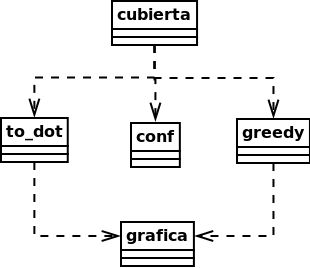
\includegraphics[width=5cm, height=5cm]{diagrama}
\end{center}

El módulo cubierta es donde se encuentra la parte principal del sistema y donde se implementa la heurísticas de Colonia de hormigas.\\
Por otro lado está el modulo $greedy$ donde se implementa el algoritmo glotón. Resulta muy pequeño a comparación del modulo cubierta.\\
Para la visualización se usó el programa dot de Graphviz pues resulta muy cómodo y las gráficas son muy entendibles que con una representación radial, además de que se ocupa mejor el espacio de la imagen generada.\\\\

\begin{center}
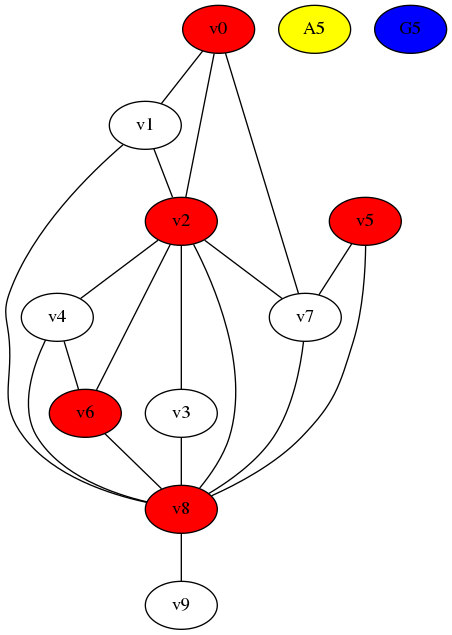
\includegraphics[width=5cm, height=5cm]{grafica_ejemplo}
\end{center}

La aplicación permite generar gráficas aleatorias o leer una gráfica de un archivo y la salida es la cubierta generada por ACO seguida por la generada con Greedy desplegadas en pantalla. Por otro lado genera un archivo con la sintaxis de dot para visualizar la gráfica.\\\\

\subsection{Resultados}
Para comparar ambos programas, se usaron gráficas de 20 vértices, pues pueden desplegarse de forma que pueden analizarse visualmente sin problemas. Se corrió con 100 gráficas diferentes y para cada gráfica se corrió el sistema ACO con 100 semillas, dando un total de 10000 experimentos. Las gráficas fueron de tamaño 25.\\\\
En cuanto a la configuración de ACO, se usaron las constante que sugiere \emph{Shyong Jian Shyu} \cite{ACOorigen}. En general no se notó un gran cambio en las soluciones variando ligeramente los valores. Dichos valores son:\\\\

\begin{center}
$\rho = 0.5 - tasa de evaporación de feromona$\\
$\tau_{0} = 13.34 - cantidad de feromona inicial$\\
$\phi = 0.6 - parámetro para ajustar la feromona$\\
$u = 5 - número de hormigas$\\
$ q_{0} = 0.9  - valor para elegir vertices$\\
$\beta = 1.0$\\
$n = 100 - Cilos que realizará el sistema $\\
\end{center}

La primera observación que se puede notar es que las soluciones entregadas por ambos sistemas son muy cercanas, variando por  lo más un vértice. La mayoría de los casos quedaban a la par, seguido por casos en los que ACO remontaba por un vértice y finalmente en los que perdía por un vértice.\\\\

Aunque logra superar la estrategia greedy con gráficas aleatorias, no basta para ver la ventaja que podría suponer ACO ante su competidor.\\\\
 
El problema que presenta la estrategia greedy es que por su misma motivación ambiciosa, puede alejarse bastante de la solución óptima. Para la siguiente prueba se construyo una gráfica de la que antemano se conocía la cubierta óptima y los vértices que la conforman se conectan a otros vértices nuevos. Esto se hace mientras el grado máximo de los vértices en la cubierta no sea mayor que el grado de los nuevos.\\\\
Con el ejemplo anterior el algoritmo glotón se deja engañar dando una solución bastante alejada de la que entrega ACO, siendo esta última la mas cercana a la óptima.\\\\

\begin{center}
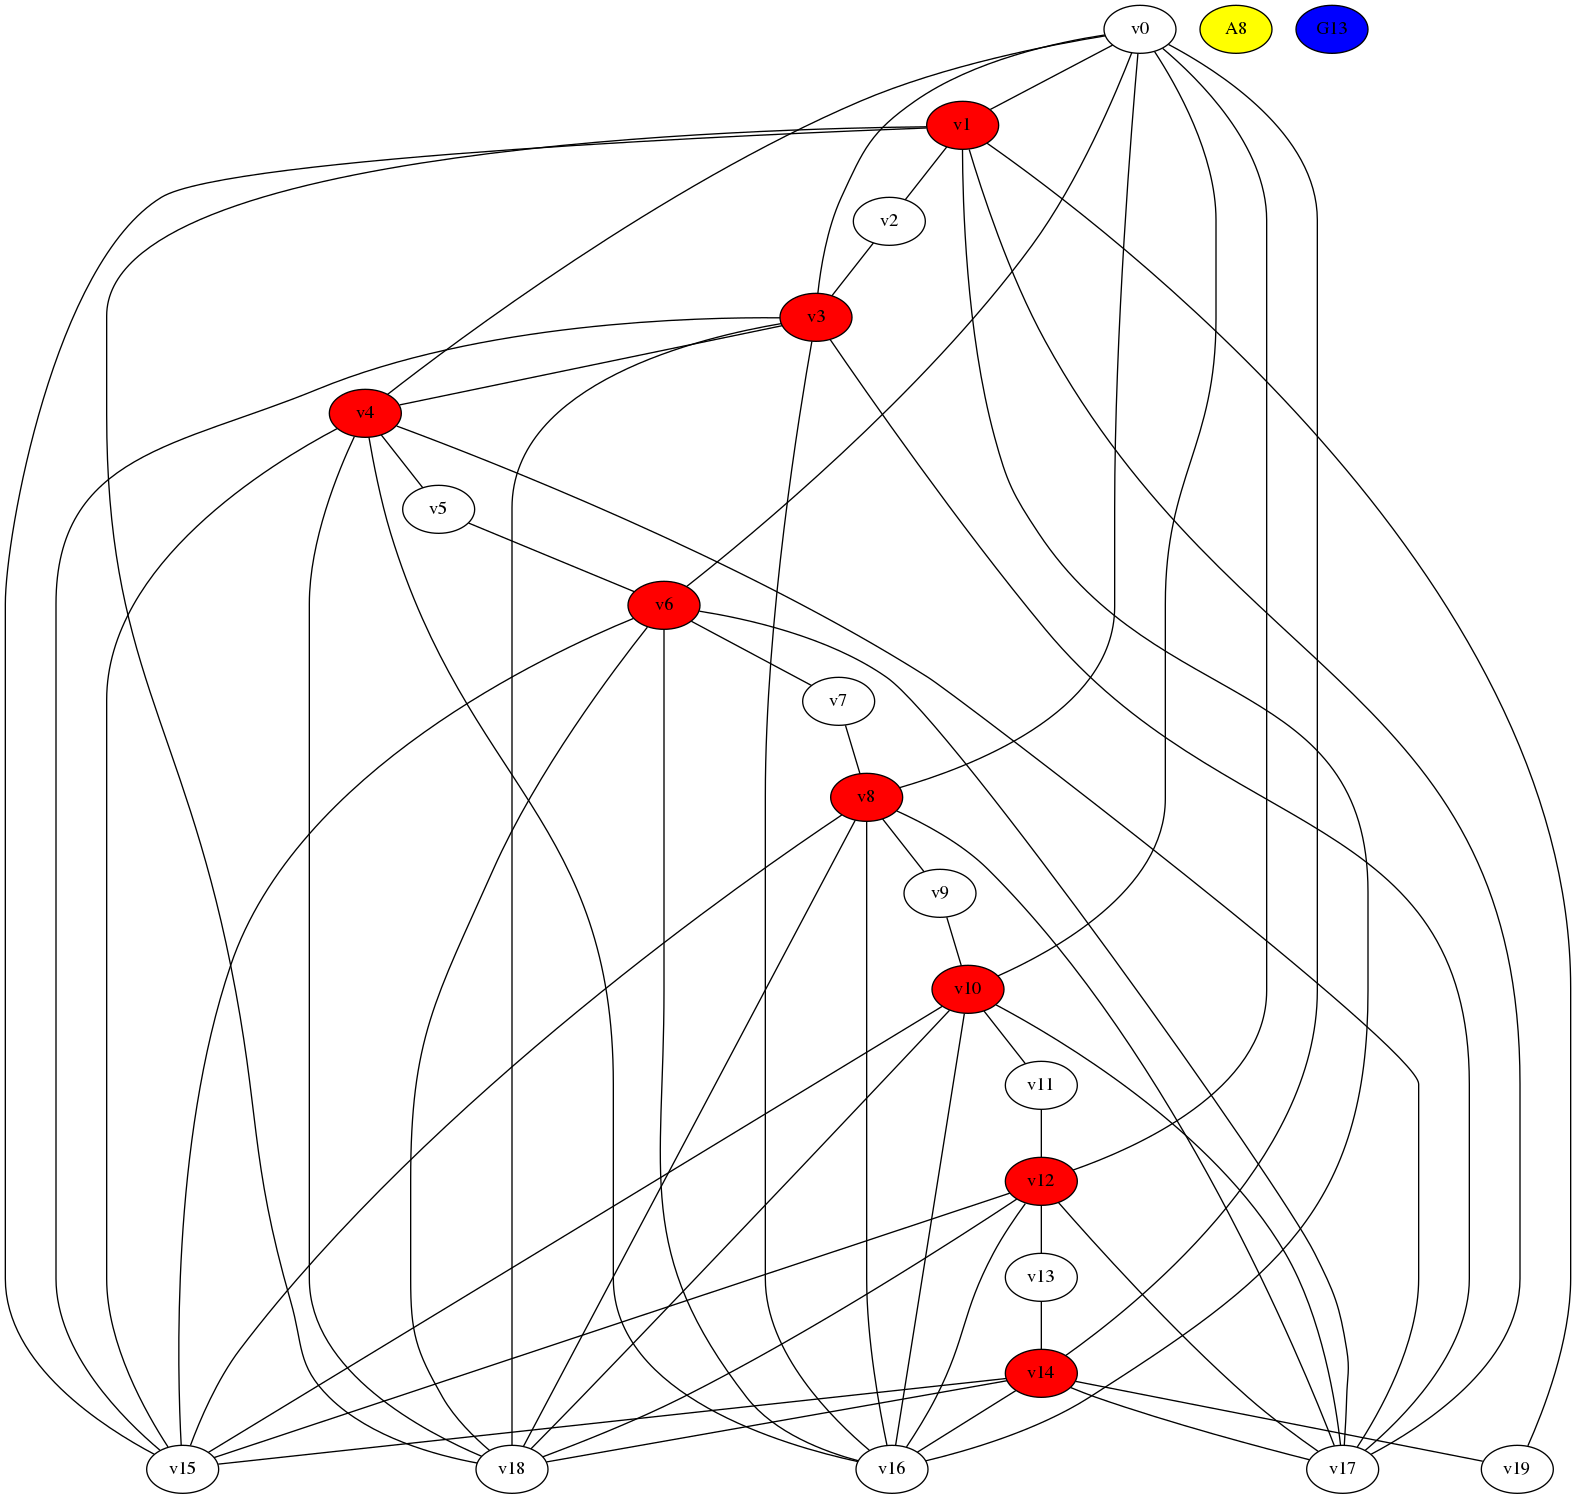
\includegraphics[width=7cm, height=7cm]{grafica_truco}
\end{center}

\section{Conclusiónes}
Si bien en el caso general resultó estar muy cerca de Greedy, en ocasiones lograba superarlo. Considero que esto se debe más a la estructura de las gráficas, pues con Gráficas Adecuadas, ACO muestra una ventaja considerable con respecto al algoritmo gloltón y siendo muy densas, dejar vértices fuera de la cubierta resulta mas complicado.\\\\

Considero que se logró el objetivo del proyecto, pues e cuenta con un sistema que entrega soluciones buenas de forma consistente a diferencia de greedy que se puede desviar bastante y no es tan fácil notar en que casos será así. Además, otro objetivo indirecto era aprender como funciona ACO en su estructura y detalles. Con ello se puede contar con otra herramienta para buscar dar solución a problemas difíciles y no tirar la toalla en cuanto estos aparecen, mejor aún dar soluciones buenas y que puedan resultar útiles en el mundo real


\begin{thebibliography}{99}	
  \bibitem{vertexcover}
  Michael R. Garey, David S. Johnson
  \emph{Computers and Intractability},
  Library of Congress Calaloging in Publication Data,
  1979,
  pp 46. 
  
  \bibitem{ACOorigen}
  Shyong Jian Shyu,
  \emph{An Ant Colony Optimization Algorithm for the Minimum Weight Vertex Cover Problem},
  Department of Computer Science and Information Engineering, Ming Chuan University,
  2004.
  
  \bibitem{ACOVC}
  https://web.archive.org/web/20041014062818/http://www.e-gold.com/unsecure/aboutus.html
  
\end{thebibliography}

\end{document}
